\section{Experimentación}

\subsection{Experimentación de performance heurísticas}

\subsubsection{Aclaraciones}

Para la siguiente experimentación, se optó por tomar dos casos distintos para graficar la performance de cada heurística:

\begin{itemize}
\item Medición de performance en base a tamaño del grafo.
\item Medición de performance en base a distribución del grafo.
\end{itemize}

\subsubsubsection{Medición en base a tamaño del grafo}
Para realizar el siguiente experimento, se tomaron datasets con distintas distribuciones del mismo tamaño y se tomó el promedio de ejecución para cada uno de ellos en base a 50 ejecuciones. En base a los resultados obtenidos, se seleccionó el mejor caso y se realizaron pruebas sobre datasets incrementando el tamaño.

\vskip 8pt

El punto de partida es un dataset de tamaño n = 45 ya que dicho tamaño se encontraba disponible para todos los tipos de datasets a experimentar.

\subsubsubsection{Medición en base a tamaño del grafo}
En base al mejor caso encontrado para el punto anterior, se utilizaron las demás instancias para mostrar como la distribución del grafo afecta la performance del mismo.

\subsubsection{Heurística constructiva de cluster-first, route-second, clusterizando con algoritmo de K-means}

\subsubsubsection{Medición en base a tamaño del grafo}

En este caso, la heurística plantea que en peor caso tendremos k clusters igual a n, con una complejidad temporal de $\mathcal{O}(n^{2} * log(n))$. Es por ello que en algunos casos podemos tener k clusters menores a n, por ello, es de esperar un gráfico con variaciones.

\begin{figure}[H]
	\centering
	\begin{minipage}[t]{.45\textwidth}
		\centering
		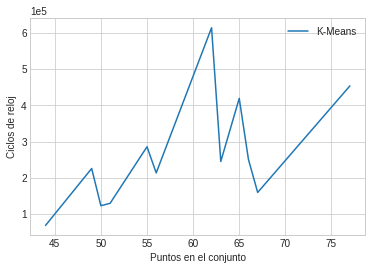
\includegraphics[scale=0.55]{exercise5/kmeans3}
	\end{minipage}\qquad
	\begin{minipage}[t]{.45\textwidth}
		\centering
		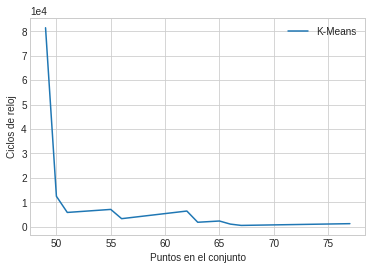
\includegraphics[scale=0.55]{exercise5/kmeansAcotado}
	\end{minipage}
\end{figure}

Tal como era de esperar, el gráfico no presenta una curva de crecimiento continuo a medida que crece el valor de n. Sin embargo, en el gráfico de la derecha vemos como la curva que representa a los puntos del gráfico del lado izquierdo, divididos por la cota de complejidad temporal, converge. Esto muestra que la heurística respeta la complejidad temproal planteada.

Luego, podemos concluir que la distribución de los puntos afecta en gran parte a la performance del algoritmo.


\subsubsubsection{Medición en base a distribución del grafo}

Dado que este algoritmo se comporta mejor en casos con clusters, se decidió comparar un caso de clusters contra otro generado aleatoriamente. Se espera que el caso generado con clusters sea más rápido.

\begin{figure}[H]
	\centering
	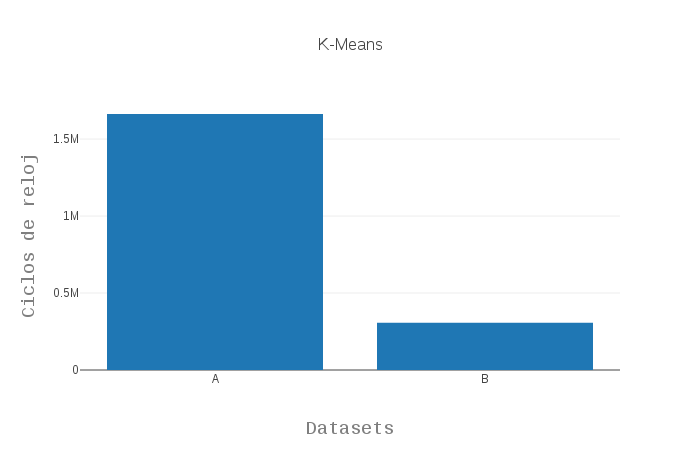
\includegraphics[scale=0.4]{exercise5/kmeansType.png}
\end{figure}

El gráfico cumple con la suposición.
\subsubsection{Heurística constructiva de cluster-first, route-second, clusterizando con algoritmo de K-means}

\subsubsubsection{Medición en base a tamaño del grafo}

En este caso, la heurística plantea que en peor caso tendremos k clusters igual a n, con una complejidad temporal de $\mathcal{O}(n^{2} * log(n))$. Es por ello que en algunos casos podemos tener k clusters menores a n, por ello, es de esperar un gráfico con variaciones.

\begin{figure}[H]
	\centering
	\begin{minipage}[t]{.45\textwidth}
		\centering
		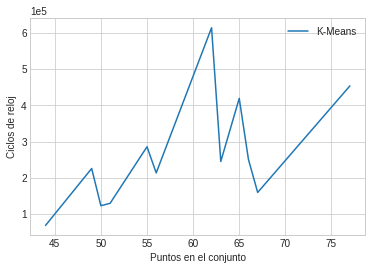
\includegraphics[scale=0.55]{exercise5/kmeans3}
	\end{minipage}\qquad
	\begin{minipage}[t]{.45\textwidth}
		\centering
		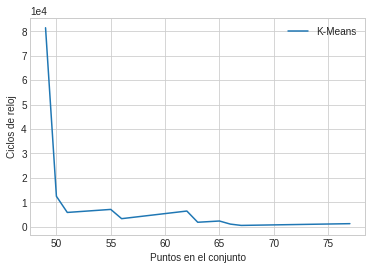
\includegraphics[scale=0.55]{exercise5/kmeansAcotado}
	\end{minipage}
\end{figure}

Tal como era de esperar, el gráfico no presenta una curva de crecimiento continuo a medida que crece el valor de n. Sin embargo, en el gráfico de la derecha vemos como la curva que representa a los puntos del gráfico del lado izquierdo, divididos por la cota de complejidad temporal, converge. Esto muestra que la heurística respeta la complejidad temproal planteada.

Luego, podemos concluir que la distribución de los puntos afecta en gran parte a la performance del algoritmo.


\subsubsubsection{Medición en base a distribución del grafo}

Dado que este algoritmo se comporta mejor en casos con clusters, se decidió comparar un caso de clusters contra otro generado aleatoriamente. Se espera que el caso generado con clusters sea más rápido.

\begin{figure}[H]
	\centering
	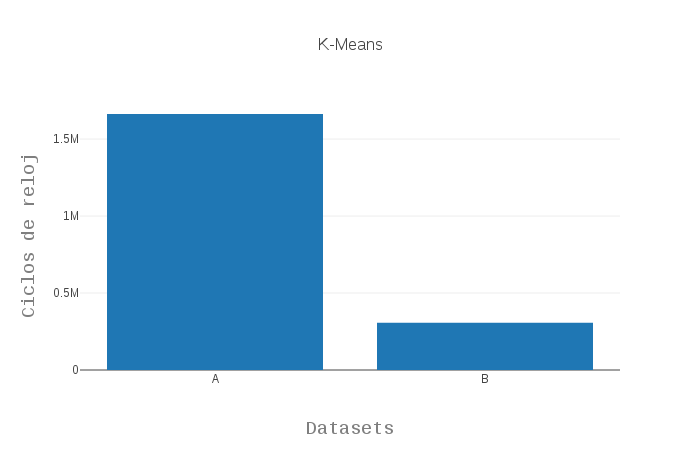
\includegraphics[scale=0.4]{exercise5/kmeansType.png}
\end{figure}

El gráfico cumple con la suposición.
\subsubsection{Heurística constructiva de cluster-first, route-second, clusterizando con algoritmo de K-means}

\subsubsubsection{Medición en base a tamaño del grafo}

En este caso, la heurística plantea que en peor caso tendremos k clusters igual a n, con una complejidad temporal de $\mathcal{O}(n^{2} * log(n))$. Es por ello que en algunos casos podemos tener k clusters menores a n, por ello, es de esperar un gráfico con variaciones.

\begin{figure}[H]
	\centering
	\begin{minipage}[t]{.45\textwidth}
		\centering
		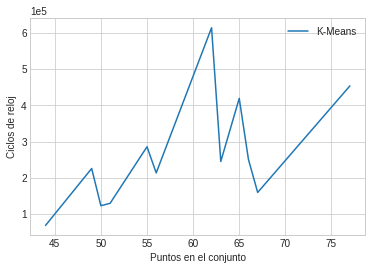
\includegraphics[scale=0.55]{exercise5/kmeans3}
	\end{minipage}\qquad
	\begin{minipage}[t]{.45\textwidth}
		\centering
		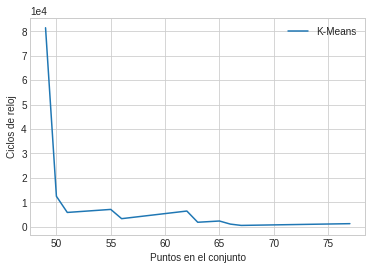
\includegraphics[scale=0.55]{exercise5/kmeansAcotado}
	\end{minipage}
\end{figure}

Tal como era de esperar, el gráfico no presenta una curva de crecimiento continuo a medida que crece el valor de n. Sin embargo, en el gráfico de la derecha vemos como la curva que representa a los puntos del gráfico del lado izquierdo, divididos por la cota de complejidad temporal, converge. Esto muestra que la heurística respeta la complejidad temproal planteada.

Luego, podemos concluir que la distribución de los puntos afecta en gran parte a la performance del algoritmo.


\subsubsubsection{Medición en base a distribución del grafo}

Dado que este algoritmo se comporta mejor en casos con clusters, se decidió comparar un caso de clusters contra otro generado aleatoriamente. Se espera que el caso generado con clusters sea más rápido.

\begin{figure}[H]
	\centering
	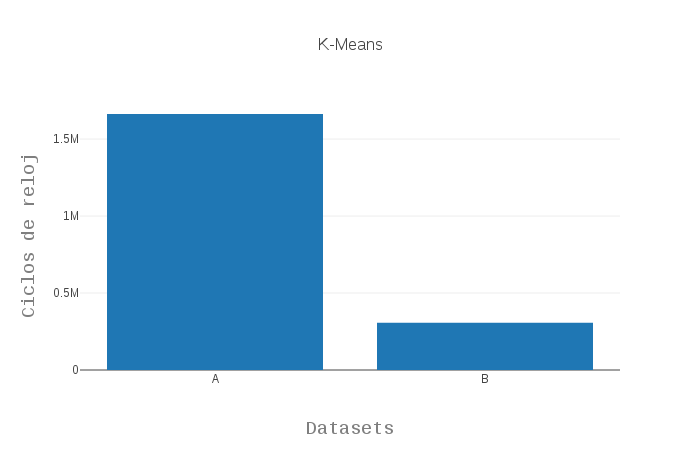
\includegraphics[scale=0.4]{exercise5/kmeansType.png}
\end{figure}

El gráfico cumple con la suposición.
\subsubsection{Heurística constructiva de cluster-first, route-second, clusterizando con algoritmo de K-means}

\subsubsubsection{Medición en base a tamaño del grafo}

En este caso, la heurística plantea que en peor caso tendremos k clusters igual a n, con una complejidad temporal de $\mathcal{O}(n^{2} * log(n))$. Es por ello que en algunos casos podemos tener k clusters menores a n, por ello, es de esperar un gráfico con variaciones.

\begin{figure}[H]
	\centering
	\begin{minipage}[t]{.45\textwidth}
		\centering
		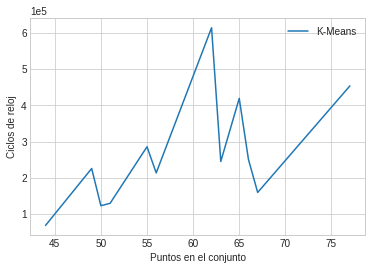
\includegraphics[scale=0.55]{exercise5/kmeans3}
	\end{minipage}\qquad
	\begin{minipage}[t]{.45\textwidth}
		\centering
		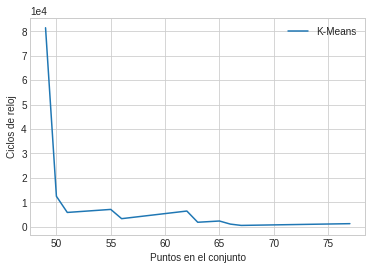
\includegraphics[scale=0.55]{exercise5/kmeansAcotado}
	\end{minipage}
\end{figure}

Tal como era de esperar, el gráfico no presenta una curva de crecimiento continuo a medida que crece el valor de n. Sin embargo, en el gráfico de la derecha vemos como la curva que representa a los puntos del gráfico del lado izquierdo, divididos por la cota de complejidad temporal, converge. Esto muestra que la heurística respeta la complejidad temproal planteada.

Luego, podemos concluir que la distribución de los puntos afecta en gran parte a la performance del algoritmo.


\subsubsubsection{Medición en base a distribución del grafo}

Dado que este algoritmo se comporta mejor en casos con clusters, se decidió comparar un caso de clusters contra otro generado aleatoriamente. Se espera que el caso generado con clusters sea más rápido.

\begin{figure}[H]
	\centering
	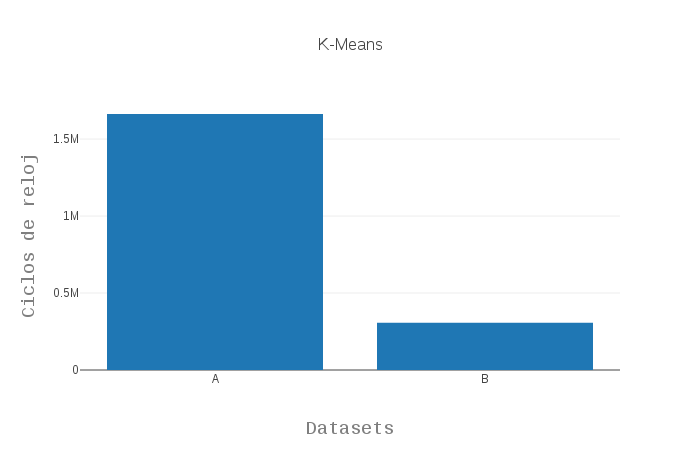
\includegraphics[scale=0.4]{exercise5/kmeansType.png}
\end{figure}

El gráfico cumple con la suposición.
\subsubsection{Heurística constructiva de cluster-first, route-second, clusterizando con algoritmo de K-means}

\subsubsubsection{Medición en base a tamaño del grafo}

En este caso, la heurística plantea que en peor caso tendremos k clusters igual a n, con una complejidad temporal de $\mathcal{O}(n^{2} * log(n))$. Es por ello que en algunos casos podemos tener k clusters menores a n, por ello, es de esperar un gráfico con variaciones.

\begin{figure}[H]
	\centering
	\begin{minipage}[t]{.45\textwidth}
		\centering
		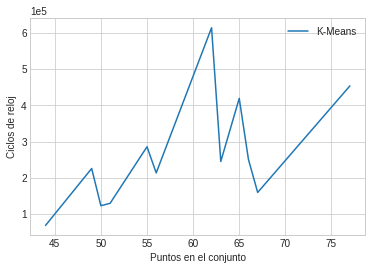
\includegraphics[scale=0.55]{exercise5/kmeans3}
	\end{minipage}\qquad
	\begin{minipage}[t]{.45\textwidth}
		\centering
		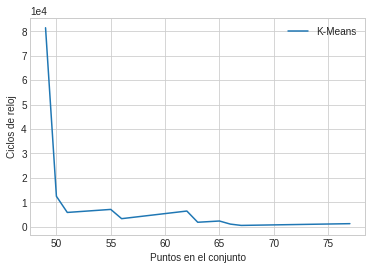
\includegraphics[scale=0.55]{exercise5/kmeansAcotado}
	\end{minipage}
\end{figure}

Tal como era de esperar, el gráfico no presenta una curva de crecimiento continuo a medida que crece el valor de n. Sin embargo, en el gráfico de la derecha vemos como la curva que representa a los puntos del gráfico del lado izquierdo, divididos por la cota de complejidad temporal, converge. Esto muestra que la heurística respeta la complejidad temproal planteada.

Luego, podemos concluir que la distribución de los puntos afecta en gran parte a la performance del algoritmo.


\subsubsubsection{Medición en base a distribución del grafo}

Dado que este algoritmo se comporta mejor en casos con clusters, se decidió comparar un caso de clusters contra otro generado aleatoriamente. Se espera que el caso generado con clusters sea más rápido.

\begin{figure}[H]
	\centering
	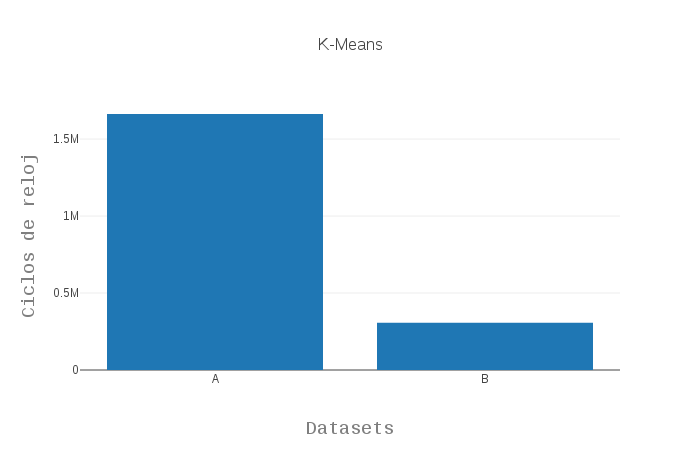
\includegraphics[scale=0.4]{exercise5/kmeansType.png}
\end{figure}

El gráfico cumple con la suposición.

<<<<<<< Updated upstream
=======
\begin{itemize}
\item Medición de performance en base a tamaño del grafo.
\item Medición de performance en base a distribución del grafo.
\end{itemize}

\subsubsection{Medición en base a tamaño del grafo}
Para realizar el siguiente experimento, se tomaron datasets con distintas distribuciones del mismo tamaño y se tomó el promedio de ejecución para cada uno de ellos en base a 50 ejecuciones. En base a los resultados obtenidos, se seleccionó el mejor caso y se realizaron pruebas sobre datasets similares, incrementando el tamaño.

\vskip 8pt

El punto de partida es un dataset de tamaño n = 45 ya que dicho tamaño se encontraba disponible para todos los tipos de datasets a experimentar.

\subsubsection{Medición en base a tamaño del grafo}
En base al mejor caso encontrado para el punto anterior, se utilizaron las demás instancias para mostrar como la distribución del grafo afecta la performance del mismo.

\section{Experimentación}

\subsection{Aclaraciones}

Para la siguiente experimentación, se optó por tomar dos casos distintos para graficar la performance de cada heurística:

\begin{itemize}
\item Medición de performance en base a tamaño del grafo.
\item Medición de performance en base a distribución del grafo.
\end{itemize}

\subsubsection{Medición en base a tamaño del grafo}
Para realizar el siguiente experimento, se tomaron datasets con distintas distribuciones del mismo tamaño y se tomó el promedio de ejecución para cada uno de ellos en base a 50 ejecuciones. En base a los resultados obtenidos, se seleccionó el mejor caso y se realizaron pruebas sobre datasets incrementando el tamaño.

\vskip 8pt

El punto de partida es un dataset de tamaño n = 45 ya que dicho tamaño se encontraba disponible para todos los tipos de datasets a experimentar.

\subsubsection{Medición en base a tamaño del grafo}
En base al mejor caso encontrado para el punto anterior, se utilizaron las demás instancias para mostrar como la distribución del grafo afecta la performance del mismo.

\section{Experimentación}

\subsection{Aclaraciones}

Para la siguiente experimentación, se optó por tomar dos casos distintos para graficar la performance de cada heurística:

\begin{itemize}
\item Medición de performance en base a tamaño del grafo.
\item Medición de performance en base a distribución del grafo.
\end{itemize}

\subsubsection{Medición en base a tamaño del grafo}
Para realizar el siguiente experimento, se tomaron datasets con distintas distribuciones del mismo tamaño y se tomó el promedio de ejecución para cada uno de ellos en base a 50 ejecuciones. En base a los resultados obtenidos, se seleccionó el mejor caso y se realizaron pruebas sobre datasets incrementando el tamaño.

\vskip 8pt

El punto de partida es un dataset de tamaño n = 45 ya que dicho tamaño se encontraba disponible para todos los tipos de datasets a experimentar.

\subsubsection{Medición en base a tamaño del grafo}
En base al mejor caso encontrado para el punto anterior, se utilizaron las demás instancias para mostrar como la distribución del grafo afecta la performance del mismo.

\section{Experimentación}

\subsection{Aclaraciones}

Para la siguiente experimentación, se optó por tomar dos casos distintos para graficar la performance de cada heurística:

\begin{itemize}
\item Medición de performance en base a tamaño del grafo.
\item Medición de performance en base a distribución del grafo.
\end{itemize}

\subsubsection{Medición en base a tamaño del grafo}
Para realizar el siguiente experimento, se tomaron datasets con distintas distribuciones del mismo tamaño y se tomó el promedio de ejecución para cada uno de ellos en base a 50 ejecuciones. En base a los resultados obtenidos, se seleccionó el mejor caso y se realizaron pruebas sobre datasets incrementando el tamaño.

\vskip 8pt

El punto de partida es un dataset de tamaño n = 45 ya que dicho tamaño se encontraba disponible para todos los tipos de datasets a experimentar.

\subsubsection{Medición en base a tamaño del grafo}
En base al mejor caso encontrado para el punto anterior, se utilizaron las demás instancias para mostrar como la distribución del grafo afecta la performance del mismo.

\input{sections/savings/experimentacion}
\input{sections/greedy/experimentacion}
\input{sections/sweep/experimentacion}
\input{sections/kmeans/experimentacion}
\input{sections/annealing/experimentacion}


\section{Experimentación}

\subsection{Aclaraciones}

Para la siguiente experimentación, se optó por tomar dos casos distintos para graficar la performance de cada heurística:

\begin{itemize}
\item Medición de performance en base a tamaño del grafo.
\item Medición de performance en base a distribución del grafo.
\end{itemize}

\subsubsection{Medición en base a tamaño del grafo}
Para realizar el siguiente experimento, se tomaron datasets con distintas distribuciones del mismo tamaño y se tomó el promedio de ejecución para cada uno de ellos en base a 50 ejecuciones. En base a los resultados obtenidos, se seleccionó el mejor caso y se realizaron pruebas sobre datasets incrementando el tamaño.

\vskip 8pt

El punto de partida es un dataset de tamaño n = 45 ya que dicho tamaño se encontraba disponible para todos los tipos de datasets a experimentar.

\subsubsection{Medición en base a tamaño del grafo}
En base al mejor caso encontrado para el punto anterior, se utilizaron las demás instancias para mostrar como la distribución del grafo afecta la performance del mismo.

\input{sections/savings/experimentacion}
\input{sections/greedy/experimentacion}
\input{sections/sweep/experimentacion}
\input{sections/kmeans/experimentacion}
\input{sections/annealing/experimentacion}


\section{Experimentación}

\subsection{Aclaraciones}

Para la siguiente experimentación, se optó por tomar dos casos distintos para graficar la performance de cada heurística:

\begin{itemize}
\item Medición de performance en base a tamaño del grafo.
\item Medición de performance en base a distribución del grafo.
\end{itemize}

\subsubsection{Medición en base a tamaño del grafo}
Para realizar el siguiente experimento, se tomaron datasets con distintas distribuciones del mismo tamaño y se tomó el promedio de ejecución para cada uno de ellos en base a 50 ejecuciones. En base a los resultados obtenidos, se seleccionó el mejor caso y se realizaron pruebas sobre datasets incrementando el tamaño.

\vskip 8pt

El punto de partida es un dataset de tamaño n = 45 ya que dicho tamaño se encontraba disponible para todos los tipos de datasets a experimentar.

\subsubsection{Medición en base a tamaño del grafo}
En base al mejor caso encontrado para el punto anterior, se utilizaron las demás instancias para mostrar como la distribución del grafo afecta la performance del mismo.

\input{sections/savings/experimentacion}
\input{sections/greedy/experimentacion}
\input{sections/sweep/experimentacion}
\input{sections/kmeans/experimentacion}
\input{sections/annealing/experimentacion}


\section{Experimentación}

\subsection{Aclaraciones}

Para la siguiente experimentación, se optó por tomar dos casos distintos para graficar la performance de cada heurística:

\begin{itemize}
\item Medición de performance en base a tamaño del grafo.
\item Medición de performance en base a distribución del grafo.
\end{itemize}

\subsubsection{Medición en base a tamaño del grafo}
Para realizar el siguiente experimento, se tomaron datasets con distintas distribuciones del mismo tamaño y se tomó el promedio de ejecución para cada uno de ellos en base a 50 ejecuciones. En base a los resultados obtenidos, se seleccionó el mejor caso y se realizaron pruebas sobre datasets incrementando el tamaño.

\vskip 8pt

El punto de partida es un dataset de tamaño n = 45 ya que dicho tamaño se encontraba disponible para todos los tipos de datasets a experimentar.

\subsubsection{Medición en base a tamaño del grafo}
En base al mejor caso encontrado para el punto anterior, se utilizaron las demás instancias para mostrar como la distribución del grafo afecta la performance del mismo.

\input{sections/savings/experimentacion}
\input{sections/greedy/experimentacion}
\input{sections/sweep/experimentacion}
\input{sections/kmeans/experimentacion}
\input{sections/annealing/experimentacion}


\section{Experimentación}

\subsection{Aclaraciones}

Para la siguiente experimentación, se optó por tomar dos casos distintos para graficar la performance de cada heurística:

\begin{itemize}
\item Medición de performance en base a tamaño del grafo.
\item Medición de performance en base a distribución del grafo.
\end{itemize}

\subsubsection{Medición en base a tamaño del grafo}
Para realizar el siguiente experimento, se tomaron datasets con distintas distribuciones del mismo tamaño y se tomó el promedio de ejecución para cada uno de ellos en base a 50 ejecuciones. En base a los resultados obtenidos, se seleccionó el mejor caso y se realizaron pruebas sobre datasets incrementando el tamaño.

\vskip 8pt

El punto de partida es un dataset de tamaño n = 45 ya que dicho tamaño se encontraba disponible para todos los tipos de datasets a experimentar.

\subsubsection{Medición en base a tamaño del grafo}
En base al mejor caso encontrado para el punto anterior, se utilizaron las demás instancias para mostrar como la distribución del grafo afecta la performance del mismo.

\input{sections/savings/experimentacion}
\input{sections/greedy/experimentacion}
\input{sections/sweep/experimentacion}
\input{sections/kmeans/experimentacion}
\input{sections/annealing/experimentacion}




\section{Experimentación}

\subsection{Aclaraciones}

Para la siguiente experimentación, se optó por tomar dos casos distintos para graficar la performance de cada heurística:

\begin{itemize}
\item Medición de performance en base a tamaño del grafo.
\item Medición de performance en base a distribución del grafo.
\end{itemize}

\subsubsection{Medición en base a tamaño del grafo}
Para realizar el siguiente experimento, se tomaron datasets con distintas distribuciones del mismo tamaño y se tomó el promedio de ejecución para cada uno de ellos en base a 50 ejecuciones. En base a los resultados obtenidos, se seleccionó el mejor caso y se realizaron pruebas sobre datasets incrementando el tamaño.

\vskip 8pt

El punto de partida es un dataset de tamaño n = 45 ya que dicho tamaño se encontraba disponible para todos los tipos de datasets a experimentar.

\subsubsection{Medición en base a tamaño del grafo}
En base al mejor caso encontrado para el punto anterior, se utilizaron las demás instancias para mostrar como la distribución del grafo afecta la performance del mismo.

\section{Experimentación}

\subsection{Aclaraciones}

Para la siguiente experimentación, se optó por tomar dos casos distintos para graficar la performance de cada heurística:

\begin{itemize}
\item Medición de performance en base a tamaño del grafo.
\item Medición de performance en base a distribución del grafo.
\end{itemize}

\subsubsection{Medición en base a tamaño del grafo}
Para realizar el siguiente experimento, se tomaron datasets con distintas distribuciones del mismo tamaño y se tomó el promedio de ejecución para cada uno de ellos en base a 50 ejecuciones. En base a los resultados obtenidos, se seleccionó el mejor caso y se realizaron pruebas sobre datasets incrementando el tamaño.

\vskip 8pt

El punto de partida es un dataset de tamaño n = 45 ya que dicho tamaño se encontraba disponible para todos los tipos de datasets a experimentar.

\subsubsection{Medición en base a tamaño del grafo}
En base al mejor caso encontrado para el punto anterior, se utilizaron las demás instancias para mostrar como la distribución del grafo afecta la performance del mismo.

\input{sections/savings/experimentacion}
\input{sections/greedy/experimentacion}
\input{sections/sweep/experimentacion}
\input{sections/kmeans/experimentacion}
\input{sections/annealing/experimentacion}


\section{Experimentación}

\subsection{Aclaraciones}

Para la siguiente experimentación, se optó por tomar dos casos distintos para graficar la performance de cada heurística:

\begin{itemize}
\item Medición de performance en base a tamaño del grafo.
\item Medición de performance en base a distribución del grafo.
\end{itemize}

\subsubsection{Medición en base a tamaño del grafo}
Para realizar el siguiente experimento, se tomaron datasets con distintas distribuciones del mismo tamaño y se tomó el promedio de ejecución para cada uno de ellos en base a 50 ejecuciones. En base a los resultados obtenidos, se seleccionó el mejor caso y se realizaron pruebas sobre datasets incrementando el tamaño.

\vskip 8pt

El punto de partida es un dataset de tamaño n = 45 ya que dicho tamaño se encontraba disponible para todos los tipos de datasets a experimentar.

\subsubsection{Medición en base a tamaño del grafo}
En base al mejor caso encontrado para el punto anterior, se utilizaron las demás instancias para mostrar como la distribución del grafo afecta la performance del mismo.

\input{sections/savings/experimentacion}
\input{sections/greedy/experimentacion}
\input{sections/sweep/experimentacion}
\input{sections/kmeans/experimentacion}
\input{sections/annealing/experimentacion}


\section{Experimentación}

\subsection{Aclaraciones}

Para la siguiente experimentación, se optó por tomar dos casos distintos para graficar la performance de cada heurística:

\begin{itemize}
\item Medición de performance en base a tamaño del grafo.
\item Medición de performance en base a distribución del grafo.
\end{itemize}

\subsubsection{Medición en base a tamaño del grafo}
Para realizar el siguiente experimento, se tomaron datasets con distintas distribuciones del mismo tamaño y se tomó el promedio de ejecución para cada uno de ellos en base a 50 ejecuciones. En base a los resultados obtenidos, se seleccionó el mejor caso y se realizaron pruebas sobre datasets incrementando el tamaño.

\vskip 8pt

El punto de partida es un dataset de tamaño n = 45 ya que dicho tamaño se encontraba disponible para todos los tipos de datasets a experimentar.

\subsubsection{Medición en base a tamaño del grafo}
En base al mejor caso encontrado para el punto anterior, se utilizaron las demás instancias para mostrar como la distribución del grafo afecta la performance del mismo.

\input{sections/savings/experimentacion}
\input{sections/greedy/experimentacion}
\input{sections/sweep/experimentacion}
\input{sections/kmeans/experimentacion}
\input{sections/annealing/experimentacion}


\section{Experimentación}

\subsection{Aclaraciones}

Para la siguiente experimentación, se optó por tomar dos casos distintos para graficar la performance de cada heurística:

\begin{itemize}
\item Medición de performance en base a tamaño del grafo.
\item Medición de performance en base a distribución del grafo.
\end{itemize}

\subsubsection{Medición en base a tamaño del grafo}
Para realizar el siguiente experimento, se tomaron datasets con distintas distribuciones del mismo tamaño y se tomó el promedio de ejecución para cada uno de ellos en base a 50 ejecuciones. En base a los resultados obtenidos, se seleccionó el mejor caso y se realizaron pruebas sobre datasets incrementando el tamaño.

\vskip 8pt

El punto de partida es un dataset de tamaño n = 45 ya que dicho tamaño se encontraba disponible para todos los tipos de datasets a experimentar.

\subsubsection{Medición en base a tamaño del grafo}
En base al mejor caso encontrado para el punto anterior, se utilizaron las demás instancias para mostrar como la distribución del grafo afecta la performance del mismo.

\input{sections/savings/experimentacion}
\input{sections/greedy/experimentacion}
\input{sections/sweep/experimentacion}
\input{sections/kmeans/experimentacion}
\input{sections/annealing/experimentacion}


\section{Experimentación}

\subsection{Aclaraciones}

Para la siguiente experimentación, se optó por tomar dos casos distintos para graficar la performance de cada heurística:

\begin{itemize}
\item Medición de performance en base a tamaño del grafo.
\item Medición de performance en base a distribución del grafo.
\end{itemize}

\subsubsection{Medición en base a tamaño del grafo}
Para realizar el siguiente experimento, se tomaron datasets con distintas distribuciones del mismo tamaño y se tomó el promedio de ejecución para cada uno de ellos en base a 50 ejecuciones. En base a los resultados obtenidos, se seleccionó el mejor caso y se realizaron pruebas sobre datasets incrementando el tamaño.

\vskip 8pt

El punto de partida es un dataset de tamaño n = 45 ya que dicho tamaño se encontraba disponible para todos los tipos de datasets a experimentar.

\subsubsection{Medición en base a tamaño del grafo}
En base al mejor caso encontrado para el punto anterior, se utilizaron las demás instancias para mostrar como la distribución del grafo afecta la performance del mismo.

\input{sections/savings/experimentacion}
\input{sections/greedy/experimentacion}
\input{sections/sweep/experimentacion}
\input{sections/kmeans/experimentacion}
\input{sections/annealing/experimentacion}




\section{Experimentación}

\subsection{Aclaraciones}

Para la siguiente experimentación, se optó por tomar dos casos distintos para graficar la performance de cada heurística:

\begin{itemize}
\item Medición de performance en base a tamaño del grafo.
\item Medición de performance en base a distribución del grafo.
\end{itemize}

\subsubsection{Medición en base a tamaño del grafo}
Para realizar el siguiente experimento, se tomaron datasets con distintas distribuciones del mismo tamaño y se tomó el promedio de ejecución para cada uno de ellos en base a 50 ejecuciones. En base a los resultados obtenidos, se seleccionó el mejor caso y se realizaron pruebas sobre datasets incrementando el tamaño.

\vskip 8pt

El punto de partida es un dataset de tamaño n = 45 ya que dicho tamaño se encontraba disponible para todos los tipos de datasets a experimentar.

\subsubsection{Medición en base a tamaño del grafo}
En base al mejor caso encontrado para el punto anterior, se utilizaron las demás instancias para mostrar como la distribución del grafo afecta la performance del mismo.

\section{Experimentación}

\subsection{Aclaraciones}

Para la siguiente experimentación, se optó por tomar dos casos distintos para graficar la performance de cada heurística:

\begin{itemize}
\item Medición de performance en base a tamaño del grafo.
\item Medición de performance en base a distribución del grafo.
\end{itemize}

\subsubsection{Medición en base a tamaño del grafo}
Para realizar el siguiente experimento, se tomaron datasets con distintas distribuciones del mismo tamaño y se tomó el promedio de ejecución para cada uno de ellos en base a 50 ejecuciones. En base a los resultados obtenidos, se seleccionó el mejor caso y se realizaron pruebas sobre datasets incrementando el tamaño.

\vskip 8pt

El punto de partida es un dataset de tamaño n = 45 ya que dicho tamaño se encontraba disponible para todos los tipos de datasets a experimentar.

\subsubsection{Medición en base a tamaño del grafo}
En base al mejor caso encontrado para el punto anterior, se utilizaron las demás instancias para mostrar como la distribución del grafo afecta la performance del mismo.

\input{sections/savings/experimentacion}
\input{sections/greedy/experimentacion}
\input{sections/sweep/experimentacion}
\input{sections/kmeans/experimentacion}
\input{sections/annealing/experimentacion}


\section{Experimentación}

\subsection{Aclaraciones}

Para la siguiente experimentación, se optó por tomar dos casos distintos para graficar la performance de cada heurística:

\begin{itemize}
\item Medición de performance en base a tamaño del grafo.
\item Medición de performance en base a distribución del grafo.
\end{itemize}

\subsubsection{Medición en base a tamaño del grafo}
Para realizar el siguiente experimento, se tomaron datasets con distintas distribuciones del mismo tamaño y se tomó el promedio de ejecución para cada uno de ellos en base a 50 ejecuciones. En base a los resultados obtenidos, se seleccionó el mejor caso y se realizaron pruebas sobre datasets incrementando el tamaño.

\vskip 8pt

El punto de partida es un dataset de tamaño n = 45 ya que dicho tamaño se encontraba disponible para todos los tipos de datasets a experimentar.

\subsubsection{Medición en base a tamaño del grafo}
En base al mejor caso encontrado para el punto anterior, se utilizaron las demás instancias para mostrar como la distribución del grafo afecta la performance del mismo.

\input{sections/savings/experimentacion}
\input{sections/greedy/experimentacion}
\input{sections/sweep/experimentacion}
\input{sections/kmeans/experimentacion}
\input{sections/annealing/experimentacion}


\section{Experimentación}

\subsection{Aclaraciones}

Para la siguiente experimentación, se optó por tomar dos casos distintos para graficar la performance de cada heurística:

\begin{itemize}
\item Medición de performance en base a tamaño del grafo.
\item Medición de performance en base a distribución del grafo.
\end{itemize}

\subsubsection{Medición en base a tamaño del grafo}
Para realizar el siguiente experimento, se tomaron datasets con distintas distribuciones del mismo tamaño y se tomó el promedio de ejecución para cada uno de ellos en base a 50 ejecuciones. En base a los resultados obtenidos, se seleccionó el mejor caso y se realizaron pruebas sobre datasets incrementando el tamaño.

\vskip 8pt

El punto de partida es un dataset de tamaño n = 45 ya que dicho tamaño se encontraba disponible para todos los tipos de datasets a experimentar.

\subsubsection{Medición en base a tamaño del grafo}
En base al mejor caso encontrado para el punto anterior, se utilizaron las demás instancias para mostrar como la distribución del grafo afecta la performance del mismo.

\input{sections/savings/experimentacion}
\input{sections/greedy/experimentacion}
\input{sections/sweep/experimentacion}
\input{sections/kmeans/experimentacion}
\input{sections/annealing/experimentacion}


\section{Experimentación}

\subsection{Aclaraciones}

Para la siguiente experimentación, se optó por tomar dos casos distintos para graficar la performance de cada heurística:

\begin{itemize}
\item Medición de performance en base a tamaño del grafo.
\item Medición de performance en base a distribución del grafo.
\end{itemize}

\subsubsection{Medición en base a tamaño del grafo}
Para realizar el siguiente experimento, se tomaron datasets con distintas distribuciones del mismo tamaño y se tomó el promedio de ejecución para cada uno de ellos en base a 50 ejecuciones. En base a los resultados obtenidos, se seleccionó el mejor caso y se realizaron pruebas sobre datasets incrementando el tamaño.

\vskip 8pt

El punto de partida es un dataset de tamaño n = 45 ya que dicho tamaño se encontraba disponible para todos los tipos de datasets a experimentar.

\subsubsection{Medición en base a tamaño del grafo}
En base al mejor caso encontrado para el punto anterior, se utilizaron las demás instancias para mostrar como la distribución del grafo afecta la performance del mismo.

\input{sections/savings/experimentacion}
\input{sections/greedy/experimentacion}
\input{sections/sweep/experimentacion}
\input{sections/kmeans/experimentacion}
\input{sections/annealing/experimentacion}


\section{Experimentación}

\subsection{Aclaraciones}

Para la siguiente experimentación, se optó por tomar dos casos distintos para graficar la performance de cada heurística:

\begin{itemize}
\item Medición de performance en base a tamaño del grafo.
\item Medición de performance en base a distribución del grafo.
\end{itemize}

\subsubsection{Medición en base a tamaño del grafo}
Para realizar el siguiente experimento, se tomaron datasets con distintas distribuciones del mismo tamaño y se tomó el promedio de ejecución para cada uno de ellos en base a 50 ejecuciones. En base a los resultados obtenidos, se seleccionó el mejor caso y se realizaron pruebas sobre datasets incrementando el tamaño.

\vskip 8pt

El punto de partida es un dataset de tamaño n = 45 ya que dicho tamaño se encontraba disponible para todos los tipos de datasets a experimentar.

\subsubsection{Medición en base a tamaño del grafo}
En base al mejor caso encontrado para el punto anterior, se utilizaron las demás instancias para mostrar como la distribución del grafo afecta la performance del mismo.

\input{sections/savings/experimentacion}
\input{sections/greedy/experimentacion}
\input{sections/sweep/experimentacion}
\input{sections/kmeans/experimentacion}
\input{sections/annealing/experimentacion}




\section{Experimentación}

\subsection{Aclaraciones}

Para la siguiente experimentación, se optó por tomar dos casos distintos para graficar la performance de cada heurística:

\begin{itemize}
\item Medición de performance en base a tamaño del grafo.
\item Medición de performance en base a distribución del grafo.
\end{itemize}

\subsubsection{Medición en base a tamaño del grafo}
Para realizar el siguiente experimento, se tomaron datasets con distintas distribuciones del mismo tamaño y se tomó el promedio de ejecución para cada uno de ellos en base a 50 ejecuciones. En base a los resultados obtenidos, se seleccionó el mejor caso y se realizaron pruebas sobre datasets incrementando el tamaño.

\vskip 8pt

El punto de partida es un dataset de tamaño n = 45 ya que dicho tamaño se encontraba disponible para todos los tipos de datasets a experimentar.

\subsubsection{Medición en base a tamaño del grafo}
En base al mejor caso encontrado para el punto anterior, se utilizaron las demás instancias para mostrar como la distribución del grafo afecta la performance del mismo.

\section{Experimentación}

\subsection{Aclaraciones}

Para la siguiente experimentación, se optó por tomar dos casos distintos para graficar la performance de cada heurística:

\begin{itemize}
\item Medición de performance en base a tamaño del grafo.
\item Medición de performance en base a distribución del grafo.
\end{itemize}

\subsubsection{Medición en base a tamaño del grafo}
Para realizar el siguiente experimento, se tomaron datasets con distintas distribuciones del mismo tamaño y se tomó el promedio de ejecución para cada uno de ellos en base a 50 ejecuciones. En base a los resultados obtenidos, se seleccionó el mejor caso y se realizaron pruebas sobre datasets incrementando el tamaño.

\vskip 8pt

El punto de partida es un dataset de tamaño n = 45 ya que dicho tamaño se encontraba disponible para todos los tipos de datasets a experimentar.

\subsubsection{Medición en base a tamaño del grafo}
En base al mejor caso encontrado para el punto anterior, se utilizaron las demás instancias para mostrar como la distribución del grafo afecta la performance del mismo.

\input{sections/savings/experimentacion}
\input{sections/greedy/experimentacion}
\input{sections/sweep/experimentacion}
\input{sections/kmeans/experimentacion}
\input{sections/annealing/experimentacion}


\section{Experimentación}

\subsection{Aclaraciones}

Para la siguiente experimentación, se optó por tomar dos casos distintos para graficar la performance de cada heurística:

\begin{itemize}
\item Medición de performance en base a tamaño del grafo.
\item Medición de performance en base a distribución del grafo.
\end{itemize}

\subsubsection{Medición en base a tamaño del grafo}
Para realizar el siguiente experimento, se tomaron datasets con distintas distribuciones del mismo tamaño y se tomó el promedio de ejecución para cada uno de ellos en base a 50 ejecuciones. En base a los resultados obtenidos, se seleccionó el mejor caso y se realizaron pruebas sobre datasets incrementando el tamaño.

\vskip 8pt

El punto de partida es un dataset de tamaño n = 45 ya que dicho tamaño se encontraba disponible para todos los tipos de datasets a experimentar.

\subsubsection{Medición en base a tamaño del grafo}
En base al mejor caso encontrado para el punto anterior, se utilizaron las demás instancias para mostrar como la distribución del grafo afecta la performance del mismo.

\input{sections/savings/experimentacion}
\input{sections/greedy/experimentacion}
\input{sections/sweep/experimentacion}
\input{sections/kmeans/experimentacion}
\input{sections/annealing/experimentacion}


\section{Experimentación}

\subsection{Aclaraciones}

Para la siguiente experimentación, se optó por tomar dos casos distintos para graficar la performance de cada heurística:

\begin{itemize}
\item Medición de performance en base a tamaño del grafo.
\item Medición de performance en base a distribución del grafo.
\end{itemize}

\subsubsection{Medición en base a tamaño del grafo}
Para realizar el siguiente experimento, se tomaron datasets con distintas distribuciones del mismo tamaño y se tomó el promedio de ejecución para cada uno de ellos en base a 50 ejecuciones. En base a los resultados obtenidos, se seleccionó el mejor caso y se realizaron pruebas sobre datasets incrementando el tamaño.

\vskip 8pt

El punto de partida es un dataset de tamaño n = 45 ya que dicho tamaño se encontraba disponible para todos los tipos de datasets a experimentar.

\subsubsection{Medición en base a tamaño del grafo}
En base al mejor caso encontrado para el punto anterior, se utilizaron las demás instancias para mostrar como la distribución del grafo afecta la performance del mismo.

\input{sections/savings/experimentacion}
\input{sections/greedy/experimentacion}
\input{sections/sweep/experimentacion}
\input{sections/kmeans/experimentacion}
\input{sections/annealing/experimentacion}


\section{Experimentación}

\subsection{Aclaraciones}

Para la siguiente experimentación, se optó por tomar dos casos distintos para graficar la performance de cada heurística:

\begin{itemize}
\item Medición de performance en base a tamaño del grafo.
\item Medición de performance en base a distribución del grafo.
\end{itemize}

\subsubsection{Medición en base a tamaño del grafo}
Para realizar el siguiente experimento, se tomaron datasets con distintas distribuciones del mismo tamaño y se tomó el promedio de ejecución para cada uno de ellos en base a 50 ejecuciones. En base a los resultados obtenidos, se seleccionó el mejor caso y se realizaron pruebas sobre datasets incrementando el tamaño.

\vskip 8pt

El punto de partida es un dataset de tamaño n = 45 ya que dicho tamaño se encontraba disponible para todos los tipos de datasets a experimentar.

\subsubsection{Medición en base a tamaño del grafo}
En base al mejor caso encontrado para el punto anterior, se utilizaron las demás instancias para mostrar como la distribución del grafo afecta la performance del mismo.

\input{sections/savings/experimentacion}
\input{sections/greedy/experimentacion}
\input{sections/sweep/experimentacion}
\input{sections/kmeans/experimentacion}
\input{sections/annealing/experimentacion}


\section{Experimentación}

\subsection{Aclaraciones}

Para la siguiente experimentación, se optó por tomar dos casos distintos para graficar la performance de cada heurística:

\begin{itemize}
\item Medición de performance en base a tamaño del grafo.
\item Medición de performance en base a distribución del grafo.
\end{itemize}

\subsubsection{Medición en base a tamaño del grafo}
Para realizar el siguiente experimento, se tomaron datasets con distintas distribuciones del mismo tamaño y se tomó el promedio de ejecución para cada uno de ellos en base a 50 ejecuciones. En base a los resultados obtenidos, se seleccionó el mejor caso y se realizaron pruebas sobre datasets incrementando el tamaño.

\vskip 8pt

El punto de partida es un dataset de tamaño n = 45 ya que dicho tamaño se encontraba disponible para todos los tipos de datasets a experimentar.

\subsubsection{Medición en base a tamaño del grafo}
En base al mejor caso encontrado para el punto anterior, se utilizaron las demás instancias para mostrar como la distribución del grafo afecta la performance del mismo.

\input{sections/savings/experimentacion}
\input{sections/greedy/experimentacion}
\input{sections/sweep/experimentacion}
\input{sections/kmeans/experimentacion}
\input{sections/annealing/experimentacion}




\section{Experimentación}

\subsection{Aclaraciones}

Para la siguiente experimentación, se optó por tomar dos casos distintos para graficar la performance de cada heurística:

\begin{itemize}
\item Medición de performance en base a tamaño del grafo.
\item Medición de performance en base a distribución del grafo.
\end{itemize}

\subsubsection{Medición en base a tamaño del grafo}
Para realizar el siguiente experimento, se tomaron datasets con distintas distribuciones del mismo tamaño y se tomó el promedio de ejecución para cada uno de ellos en base a 50 ejecuciones. En base a los resultados obtenidos, se seleccionó el mejor caso y se realizaron pruebas sobre datasets incrementando el tamaño.

\vskip 8pt

El punto de partida es un dataset de tamaño n = 45 ya que dicho tamaño se encontraba disponible para todos los tipos de datasets a experimentar.

\subsubsection{Medición en base a tamaño del grafo}
En base al mejor caso encontrado para el punto anterior, se utilizaron las demás instancias para mostrar como la distribución del grafo afecta la performance del mismo.

\section{Experimentación}

\subsection{Aclaraciones}

Para la siguiente experimentación, se optó por tomar dos casos distintos para graficar la performance de cada heurística:

\begin{itemize}
\item Medición de performance en base a tamaño del grafo.
\item Medición de performance en base a distribución del grafo.
\end{itemize}

\subsubsection{Medición en base a tamaño del grafo}
Para realizar el siguiente experimento, se tomaron datasets con distintas distribuciones del mismo tamaño y se tomó el promedio de ejecución para cada uno de ellos en base a 50 ejecuciones. En base a los resultados obtenidos, se seleccionó el mejor caso y se realizaron pruebas sobre datasets incrementando el tamaño.

\vskip 8pt

El punto de partida es un dataset de tamaño n = 45 ya que dicho tamaño se encontraba disponible para todos los tipos de datasets a experimentar.

\subsubsection{Medición en base a tamaño del grafo}
En base al mejor caso encontrado para el punto anterior, se utilizaron las demás instancias para mostrar como la distribución del grafo afecta la performance del mismo.

\input{sections/savings/experimentacion}
\input{sections/greedy/experimentacion}
\input{sections/sweep/experimentacion}
\input{sections/kmeans/experimentacion}
\input{sections/annealing/experimentacion}


\section{Experimentación}

\subsection{Aclaraciones}

Para la siguiente experimentación, se optó por tomar dos casos distintos para graficar la performance de cada heurística:

\begin{itemize}
\item Medición de performance en base a tamaño del grafo.
\item Medición de performance en base a distribución del grafo.
\end{itemize}

\subsubsection{Medición en base a tamaño del grafo}
Para realizar el siguiente experimento, se tomaron datasets con distintas distribuciones del mismo tamaño y se tomó el promedio de ejecución para cada uno de ellos en base a 50 ejecuciones. En base a los resultados obtenidos, se seleccionó el mejor caso y se realizaron pruebas sobre datasets incrementando el tamaño.

\vskip 8pt

El punto de partida es un dataset de tamaño n = 45 ya que dicho tamaño se encontraba disponible para todos los tipos de datasets a experimentar.

\subsubsection{Medición en base a tamaño del grafo}
En base al mejor caso encontrado para el punto anterior, se utilizaron las demás instancias para mostrar como la distribución del grafo afecta la performance del mismo.

\input{sections/savings/experimentacion}
\input{sections/greedy/experimentacion}
\input{sections/sweep/experimentacion}
\input{sections/kmeans/experimentacion}
\input{sections/annealing/experimentacion}


\section{Experimentación}

\subsection{Aclaraciones}

Para la siguiente experimentación, se optó por tomar dos casos distintos para graficar la performance de cada heurística:

\begin{itemize}
\item Medición de performance en base a tamaño del grafo.
\item Medición de performance en base a distribución del grafo.
\end{itemize}

\subsubsection{Medición en base a tamaño del grafo}
Para realizar el siguiente experimento, se tomaron datasets con distintas distribuciones del mismo tamaño y se tomó el promedio de ejecución para cada uno de ellos en base a 50 ejecuciones. En base a los resultados obtenidos, se seleccionó el mejor caso y se realizaron pruebas sobre datasets incrementando el tamaño.

\vskip 8pt

El punto de partida es un dataset de tamaño n = 45 ya que dicho tamaño se encontraba disponible para todos los tipos de datasets a experimentar.

\subsubsection{Medición en base a tamaño del grafo}
En base al mejor caso encontrado para el punto anterior, se utilizaron las demás instancias para mostrar como la distribución del grafo afecta la performance del mismo.

\input{sections/savings/experimentacion}
\input{sections/greedy/experimentacion}
\input{sections/sweep/experimentacion}
\input{sections/kmeans/experimentacion}
\input{sections/annealing/experimentacion}


\section{Experimentación}

\subsection{Aclaraciones}

Para la siguiente experimentación, se optó por tomar dos casos distintos para graficar la performance de cada heurística:

\begin{itemize}
\item Medición de performance en base a tamaño del grafo.
\item Medición de performance en base a distribución del grafo.
\end{itemize}

\subsubsection{Medición en base a tamaño del grafo}
Para realizar el siguiente experimento, se tomaron datasets con distintas distribuciones del mismo tamaño y se tomó el promedio de ejecución para cada uno de ellos en base a 50 ejecuciones. En base a los resultados obtenidos, se seleccionó el mejor caso y se realizaron pruebas sobre datasets incrementando el tamaño.

\vskip 8pt

El punto de partida es un dataset de tamaño n = 45 ya que dicho tamaño se encontraba disponible para todos los tipos de datasets a experimentar.

\subsubsection{Medición en base a tamaño del grafo}
En base al mejor caso encontrado para el punto anterior, se utilizaron las demás instancias para mostrar como la distribución del grafo afecta la performance del mismo.

\input{sections/savings/experimentacion}
\input{sections/greedy/experimentacion}
\input{sections/sweep/experimentacion}
\input{sections/kmeans/experimentacion}
\input{sections/annealing/experimentacion}


\section{Experimentación}

\subsection{Aclaraciones}

Para la siguiente experimentación, se optó por tomar dos casos distintos para graficar la performance de cada heurística:

\begin{itemize}
\item Medición de performance en base a tamaño del grafo.
\item Medición de performance en base a distribución del grafo.
\end{itemize}

\subsubsection{Medición en base a tamaño del grafo}
Para realizar el siguiente experimento, se tomaron datasets con distintas distribuciones del mismo tamaño y se tomó el promedio de ejecución para cada uno de ellos en base a 50 ejecuciones. En base a los resultados obtenidos, se seleccionó el mejor caso y se realizaron pruebas sobre datasets incrementando el tamaño.

\vskip 8pt

El punto de partida es un dataset de tamaño n = 45 ya que dicho tamaño se encontraba disponible para todos los tipos de datasets a experimentar.

\subsubsection{Medición en base a tamaño del grafo}
En base al mejor caso encontrado para el punto anterior, se utilizaron las demás instancias para mostrar como la distribución del grafo afecta la performance del mismo.

\input{sections/savings/experimentacion}
\input{sections/greedy/experimentacion}
\input{sections/sweep/experimentacion}
\input{sections/kmeans/experimentacion}
\input{sections/annealing/experimentacion}






\section{Experimentación}

\subsection{Aclaraciones}

Para la siguiente experimentación, se optó por tomar dos casos distintos para graficar la performance de cada heurística:

\begin{itemize}
\item Medición de performance en base a tamaño del grafo.
\item Medición de performance en base a distribución del grafo.
\end{itemize}

\subsubsection{Medición en base a tamaño del grafo}
Para realizar el siguiente experimento, se tomaron datasets con distintas distribuciones del mismo tamaño y se tomó el promedio de ejecución para cada uno de ellos en base a 50 ejecuciones. En base a los resultados obtenidos, se seleccionó el mejor caso y se realizaron pruebas sobre datasets incrementando el tamaño.

\vskip 8pt

El punto de partida es un dataset de tamaño n = 45 ya que dicho tamaño se encontraba disponible para todos los tipos de datasets a experimentar.

\subsubsection{Medición en base a tamaño del grafo}
En base al mejor caso encontrado para el punto anterior, se utilizaron las demás instancias para mostrar como la distribución del grafo afecta la performance del mismo.

\section{Experimentación}

\subsection{Aclaraciones}

Para la siguiente experimentación, se optó por tomar dos casos distintos para graficar la performance de cada heurística:

\begin{itemize}
\item Medición de performance en base a tamaño del grafo.
\item Medición de performance en base a distribución del grafo.
\end{itemize}

\subsubsection{Medición en base a tamaño del grafo}
Para realizar el siguiente experimento, se tomaron datasets con distintas distribuciones del mismo tamaño y se tomó el promedio de ejecución para cada uno de ellos en base a 50 ejecuciones. En base a los resultados obtenidos, se seleccionó el mejor caso y se realizaron pruebas sobre datasets incrementando el tamaño.

\vskip 8pt

El punto de partida es un dataset de tamaño n = 45 ya que dicho tamaño se encontraba disponible para todos los tipos de datasets a experimentar.

\subsubsection{Medición en base a tamaño del grafo}
En base al mejor caso encontrado para el punto anterior, se utilizaron las demás instancias para mostrar como la distribución del grafo afecta la performance del mismo.

\section{Experimentación}

\subsection{Aclaraciones}

Para la siguiente experimentación, se optó por tomar dos casos distintos para graficar la performance de cada heurística:

\begin{itemize}
\item Medición de performance en base a tamaño del grafo.
\item Medición de performance en base a distribución del grafo.
\end{itemize}

\subsubsection{Medición en base a tamaño del grafo}
Para realizar el siguiente experimento, se tomaron datasets con distintas distribuciones del mismo tamaño y se tomó el promedio de ejecución para cada uno de ellos en base a 50 ejecuciones. En base a los resultados obtenidos, se seleccionó el mejor caso y se realizaron pruebas sobre datasets incrementando el tamaño.

\vskip 8pt

El punto de partida es un dataset de tamaño n = 45 ya que dicho tamaño se encontraba disponible para todos los tipos de datasets a experimentar.

\subsubsection{Medición en base a tamaño del grafo}
En base al mejor caso encontrado para el punto anterior, se utilizaron las demás instancias para mostrar como la distribución del grafo afecta la performance del mismo.

\input{sections/savings/experimentacion}
\input{sections/greedy/experimentacion}
\input{sections/sweep/experimentacion}
\input{sections/kmeans/experimentacion}
\input{sections/annealing/experimentacion}


\section{Experimentación}

\subsection{Aclaraciones}

Para la siguiente experimentación, se optó por tomar dos casos distintos para graficar la performance de cada heurística:

\begin{itemize}
\item Medición de performance en base a tamaño del grafo.
\item Medición de performance en base a distribución del grafo.
\end{itemize}

\subsubsection{Medición en base a tamaño del grafo}
Para realizar el siguiente experimento, se tomaron datasets con distintas distribuciones del mismo tamaño y se tomó el promedio de ejecución para cada uno de ellos en base a 50 ejecuciones. En base a los resultados obtenidos, se seleccionó el mejor caso y se realizaron pruebas sobre datasets incrementando el tamaño.

\vskip 8pt

El punto de partida es un dataset de tamaño n = 45 ya que dicho tamaño se encontraba disponible para todos los tipos de datasets a experimentar.

\subsubsection{Medición en base a tamaño del grafo}
En base al mejor caso encontrado para el punto anterior, se utilizaron las demás instancias para mostrar como la distribución del grafo afecta la performance del mismo.

\input{sections/savings/experimentacion}
\input{sections/greedy/experimentacion}
\input{sections/sweep/experimentacion}
\input{sections/kmeans/experimentacion}
\input{sections/annealing/experimentacion}


\section{Experimentación}

\subsection{Aclaraciones}

Para la siguiente experimentación, se optó por tomar dos casos distintos para graficar la performance de cada heurística:

\begin{itemize}
\item Medición de performance en base a tamaño del grafo.
\item Medición de performance en base a distribución del grafo.
\end{itemize}

\subsubsection{Medición en base a tamaño del grafo}
Para realizar el siguiente experimento, se tomaron datasets con distintas distribuciones del mismo tamaño y se tomó el promedio de ejecución para cada uno de ellos en base a 50 ejecuciones. En base a los resultados obtenidos, se seleccionó el mejor caso y se realizaron pruebas sobre datasets incrementando el tamaño.

\vskip 8pt

El punto de partida es un dataset de tamaño n = 45 ya que dicho tamaño se encontraba disponible para todos los tipos de datasets a experimentar.

\subsubsection{Medición en base a tamaño del grafo}
En base al mejor caso encontrado para el punto anterior, se utilizaron las demás instancias para mostrar como la distribución del grafo afecta la performance del mismo.

\input{sections/savings/experimentacion}
\input{sections/greedy/experimentacion}
\input{sections/sweep/experimentacion}
\input{sections/kmeans/experimentacion}
\input{sections/annealing/experimentacion}


\section{Experimentación}

\subsection{Aclaraciones}

Para la siguiente experimentación, se optó por tomar dos casos distintos para graficar la performance de cada heurística:

\begin{itemize}
\item Medición de performance en base a tamaño del grafo.
\item Medición de performance en base a distribución del grafo.
\end{itemize}

\subsubsection{Medición en base a tamaño del grafo}
Para realizar el siguiente experimento, se tomaron datasets con distintas distribuciones del mismo tamaño y se tomó el promedio de ejecución para cada uno de ellos en base a 50 ejecuciones. En base a los resultados obtenidos, se seleccionó el mejor caso y se realizaron pruebas sobre datasets incrementando el tamaño.

\vskip 8pt

El punto de partida es un dataset de tamaño n = 45 ya que dicho tamaño se encontraba disponible para todos los tipos de datasets a experimentar.

\subsubsection{Medición en base a tamaño del grafo}
En base al mejor caso encontrado para el punto anterior, se utilizaron las demás instancias para mostrar como la distribución del grafo afecta la performance del mismo.

\input{sections/savings/experimentacion}
\input{sections/greedy/experimentacion}
\input{sections/sweep/experimentacion}
\input{sections/kmeans/experimentacion}
\input{sections/annealing/experimentacion}


\section{Experimentación}

\subsection{Aclaraciones}

Para la siguiente experimentación, se optó por tomar dos casos distintos para graficar la performance de cada heurística:

\begin{itemize}
\item Medición de performance en base a tamaño del grafo.
\item Medición de performance en base a distribución del grafo.
\end{itemize}

\subsubsection{Medición en base a tamaño del grafo}
Para realizar el siguiente experimento, se tomaron datasets con distintas distribuciones del mismo tamaño y se tomó el promedio de ejecución para cada uno de ellos en base a 50 ejecuciones. En base a los resultados obtenidos, se seleccionó el mejor caso y se realizaron pruebas sobre datasets incrementando el tamaño.

\vskip 8pt

El punto de partida es un dataset de tamaño n = 45 ya que dicho tamaño se encontraba disponible para todos los tipos de datasets a experimentar.

\subsubsection{Medición en base a tamaño del grafo}
En base al mejor caso encontrado para el punto anterior, se utilizaron las demás instancias para mostrar como la distribución del grafo afecta la performance del mismo.

\input{sections/savings/experimentacion}
\input{sections/greedy/experimentacion}
\input{sections/sweep/experimentacion}
\input{sections/kmeans/experimentacion}
\input{sections/annealing/experimentacion}




\section{Experimentación}

\subsection{Aclaraciones}

Para la siguiente experimentación, se optó por tomar dos casos distintos para graficar la performance de cada heurística:

\begin{itemize}
\item Medición de performance en base a tamaño del grafo.
\item Medición de performance en base a distribución del grafo.
\end{itemize}

\subsubsection{Medición en base a tamaño del grafo}
Para realizar el siguiente experimento, se tomaron datasets con distintas distribuciones del mismo tamaño y se tomó el promedio de ejecución para cada uno de ellos en base a 50 ejecuciones. En base a los resultados obtenidos, se seleccionó el mejor caso y se realizaron pruebas sobre datasets incrementando el tamaño.

\vskip 8pt

El punto de partida es un dataset de tamaño n = 45 ya que dicho tamaño se encontraba disponible para todos los tipos de datasets a experimentar.

\subsubsection{Medición en base a tamaño del grafo}
En base al mejor caso encontrado para el punto anterior, se utilizaron las demás instancias para mostrar como la distribución del grafo afecta la performance del mismo.

\section{Experimentación}

\subsection{Aclaraciones}

Para la siguiente experimentación, se optó por tomar dos casos distintos para graficar la performance de cada heurística:

\begin{itemize}
\item Medición de performance en base a tamaño del grafo.
\item Medición de performance en base a distribución del grafo.
\end{itemize}

\subsubsection{Medición en base a tamaño del grafo}
Para realizar el siguiente experimento, se tomaron datasets con distintas distribuciones del mismo tamaño y se tomó el promedio de ejecución para cada uno de ellos en base a 50 ejecuciones. En base a los resultados obtenidos, se seleccionó el mejor caso y se realizaron pruebas sobre datasets incrementando el tamaño.

\vskip 8pt

El punto de partida es un dataset de tamaño n = 45 ya que dicho tamaño se encontraba disponible para todos los tipos de datasets a experimentar.

\subsubsection{Medición en base a tamaño del grafo}
En base al mejor caso encontrado para el punto anterior, se utilizaron las demás instancias para mostrar como la distribución del grafo afecta la performance del mismo.

\input{sections/savings/experimentacion}
\input{sections/greedy/experimentacion}
\input{sections/sweep/experimentacion}
\input{sections/kmeans/experimentacion}
\input{sections/annealing/experimentacion}


\section{Experimentación}

\subsection{Aclaraciones}

Para la siguiente experimentación, se optó por tomar dos casos distintos para graficar la performance de cada heurística:

\begin{itemize}
\item Medición de performance en base a tamaño del grafo.
\item Medición de performance en base a distribución del grafo.
\end{itemize}

\subsubsection{Medición en base a tamaño del grafo}
Para realizar el siguiente experimento, se tomaron datasets con distintas distribuciones del mismo tamaño y se tomó el promedio de ejecución para cada uno de ellos en base a 50 ejecuciones. En base a los resultados obtenidos, se seleccionó el mejor caso y se realizaron pruebas sobre datasets incrementando el tamaño.

\vskip 8pt

El punto de partida es un dataset de tamaño n = 45 ya que dicho tamaño se encontraba disponible para todos los tipos de datasets a experimentar.

\subsubsection{Medición en base a tamaño del grafo}
En base al mejor caso encontrado para el punto anterior, se utilizaron las demás instancias para mostrar como la distribución del grafo afecta la performance del mismo.

\input{sections/savings/experimentacion}
\input{sections/greedy/experimentacion}
\input{sections/sweep/experimentacion}
\input{sections/kmeans/experimentacion}
\input{sections/annealing/experimentacion}


\section{Experimentación}

\subsection{Aclaraciones}

Para la siguiente experimentación, se optó por tomar dos casos distintos para graficar la performance de cada heurística:

\begin{itemize}
\item Medición de performance en base a tamaño del grafo.
\item Medición de performance en base a distribución del grafo.
\end{itemize}

\subsubsection{Medición en base a tamaño del grafo}
Para realizar el siguiente experimento, se tomaron datasets con distintas distribuciones del mismo tamaño y se tomó el promedio de ejecución para cada uno de ellos en base a 50 ejecuciones. En base a los resultados obtenidos, se seleccionó el mejor caso y se realizaron pruebas sobre datasets incrementando el tamaño.

\vskip 8pt

El punto de partida es un dataset de tamaño n = 45 ya que dicho tamaño se encontraba disponible para todos los tipos de datasets a experimentar.

\subsubsection{Medición en base a tamaño del grafo}
En base al mejor caso encontrado para el punto anterior, se utilizaron las demás instancias para mostrar como la distribución del grafo afecta la performance del mismo.

\input{sections/savings/experimentacion}
\input{sections/greedy/experimentacion}
\input{sections/sweep/experimentacion}
\input{sections/kmeans/experimentacion}
\input{sections/annealing/experimentacion}


\section{Experimentación}

\subsection{Aclaraciones}

Para la siguiente experimentación, se optó por tomar dos casos distintos para graficar la performance de cada heurística:

\begin{itemize}
\item Medición de performance en base a tamaño del grafo.
\item Medición de performance en base a distribución del grafo.
\end{itemize}

\subsubsection{Medición en base a tamaño del grafo}
Para realizar el siguiente experimento, se tomaron datasets con distintas distribuciones del mismo tamaño y se tomó el promedio de ejecución para cada uno de ellos en base a 50 ejecuciones. En base a los resultados obtenidos, se seleccionó el mejor caso y se realizaron pruebas sobre datasets incrementando el tamaño.

\vskip 8pt

El punto de partida es un dataset de tamaño n = 45 ya que dicho tamaño se encontraba disponible para todos los tipos de datasets a experimentar.

\subsubsection{Medición en base a tamaño del grafo}
En base al mejor caso encontrado para el punto anterior, se utilizaron las demás instancias para mostrar como la distribución del grafo afecta la performance del mismo.

\input{sections/savings/experimentacion}
\input{sections/greedy/experimentacion}
\input{sections/sweep/experimentacion}
\input{sections/kmeans/experimentacion}
\input{sections/annealing/experimentacion}


\section{Experimentación}

\subsection{Aclaraciones}

Para la siguiente experimentación, se optó por tomar dos casos distintos para graficar la performance de cada heurística:

\begin{itemize}
\item Medición de performance en base a tamaño del grafo.
\item Medición de performance en base a distribución del grafo.
\end{itemize}

\subsubsection{Medición en base a tamaño del grafo}
Para realizar el siguiente experimento, se tomaron datasets con distintas distribuciones del mismo tamaño y se tomó el promedio de ejecución para cada uno de ellos en base a 50 ejecuciones. En base a los resultados obtenidos, se seleccionó el mejor caso y se realizaron pruebas sobre datasets incrementando el tamaño.

\vskip 8pt

El punto de partida es un dataset de tamaño n = 45 ya que dicho tamaño se encontraba disponible para todos los tipos de datasets a experimentar.

\subsubsection{Medición en base a tamaño del grafo}
En base al mejor caso encontrado para el punto anterior, se utilizaron las demás instancias para mostrar como la distribución del grafo afecta la performance del mismo.

\input{sections/savings/experimentacion}
\input{sections/greedy/experimentacion}
\input{sections/sweep/experimentacion}
\input{sections/kmeans/experimentacion}
\input{sections/annealing/experimentacion}




\section{Experimentación}

\subsection{Aclaraciones}

Para la siguiente experimentación, se optó por tomar dos casos distintos para graficar la performance de cada heurística:

\begin{itemize}
\item Medición de performance en base a tamaño del grafo.
\item Medición de performance en base a distribución del grafo.
\end{itemize}

\subsubsection{Medición en base a tamaño del grafo}
Para realizar el siguiente experimento, se tomaron datasets con distintas distribuciones del mismo tamaño y se tomó el promedio de ejecución para cada uno de ellos en base a 50 ejecuciones. En base a los resultados obtenidos, se seleccionó el mejor caso y se realizaron pruebas sobre datasets incrementando el tamaño.

\vskip 8pt

El punto de partida es un dataset de tamaño n = 45 ya que dicho tamaño se encontraba disponible para todos los tipos de datasets a experimentar.

\subsubsection{Medición en base a tamaño del grafo}
En base al mejor caso encontrado para el punto anterior, se utilizaron las demás instancias para mostrar como la distribución del grafo afecta la performance del mismo.

\section{Experimentación}

\subsection{Aclaraciones}

Para la siguiente experimentación, se optó por tomar dos casos distintos para graficar la performance de cada heurística:

\begin{itemize}
\item Medición de performance en base a tamaño del grafo.
\item Medición de performance en base a distribución del grafo.
\end{itemize}

\subsubsection{Medición en base a tamaño del grafo}
Para realizar el siguiente experimento, se tomaron datasets con distintas distribuciones del mismo tamaño y se tomó el promedio de ejecución para cada uno de ellos en base a 50 ejecuciones. En base a los resultados obtenidos, se seleccionó el mejor caso y se realizaron pruebas sobre datasets incrementando el tamaño.

\vskip 8pt

El punto de partida es un dataset de tamaño n = 45 ya que dicho tamaño se encontraba disponible para todos los tipos de datasets a experimentar.

\subsubsection{Medición en base a tamaño del grafo}
En base al mejor caso encontrado para el punto anterior, se utilizaron las demás instancias para mostrar como la distribución del grafo afecta la performance del mismo.

\input{sections/savings/experimentacion}
\input{sections/greedy/experimentacion}
\input{sections/sweep/experimentacion}
\input{sections/kmeans/experimentacion}
\input{sections/annealing/experimentacion}


\section{Experimentación}

\subsection{Aclaraciones}

Para la siguiente experimentación, se optó por tomar dos casos distintos para graficar la performance de cada heurística:

\begin{itemize}
\item Medición de performance en base a tamaño del grafo.
\item Medición de performance en base a distribución del grafo.
\end{itemize}

\subsubsection{Medición en base a tamaño del grafo}
Para realizar el siguiente experimento, se tomaron datasets con distintas distribuciones del mismo tamaño y se tomó el promedio de ejecución para cada uno de ellos en base a 50 ejecuciones. En base a los resultados obtenidos, se seleccionó el mejor caso y se realizaron pruebas sobre datasets incrementando el tamaño.

\vskip 8pt

El punto de partida es un dataset de tamaño n = 45 ya que dicho tamaño se encontraba disponible para todos los tipos de datasets a experimentar.

\subsubsection{Medición en base a tamaño del grafo}
En base al mejor caso encontrado para el punto anterior, se utilizaron las demás instancias para mostrar como la distribución del grafo afecta la performance del mismo.

\input{sections/savings/experimentacion}
\input{sections/greedy/experimentacion}
\input{sections/sweep/experimentacion}
\input{sections/kmeans/experimentacion}
\input{sections/annealing/experimentacion}


\section{Experimentación}

\subsection{Aclaraciones}

Para la siguiente experimentación, se optó por tomar dos casos distintos para graficar la performance de cada heurística:

\begin{itemize}
\item Medición de performance en base a tamaño del grafo.
\item Medición de performance en base a distribución del grafo.
\end{itemize}

\subsubsection{Medición en base a tamaño del grafo}
Para realizar el siguiente experimento, se tomaron datasets con distintas distribuciones del mismo tamaño y se tomó el promedio de ejecución para cada uno de ellos en base a 50 ejecuciones. En base a los resultados obtenidos, se seleccionó el mejor caso y se realizaron pruebas sobre datasets incrementando el tamaño.

\vskip 8pt

El punto de partida es un dataset de tamaño n = 45 ya que dicho tamaño se encontraba disponible para todos los tipos de datasets a experimentar.

\subsubsection{Medición en base a tamaño del grafo}
En base al mejor caso encontrado para el punto anterior, se utilizaron las demás instancias para mostrar como la distribución del grafo afecta la performance del mismo.

\input{sections/savings/experimentacion}
\input{sections/greedy/experimentacion}
\input{sections/sweep/experimentacion}
\input{sections/kmeans/experimentacion}
\input{sections/annealing/experimentacion}


\section{Experimentación}

\subsection{Aclaraciones}

Para la siguiente experimentación, se optó por tomar dos casos distintos para graficar la performance de cada heurística:

\begin{itemize}
\item Medición de performance en base a tamaño del grafo.
\item Medición de performance en base a distribución del grafo.
\end{itemize}

\subsubsection{Medición en base a tamaño del grafo}
Para realizar el siguiente experimento, se tomaron datasets con distintas distribuciones del mismo tamaño y se tomó el promedio de ejecución para cada uno de ellos en base a 50 ejecuciones. En base a los resultados obtenidos, se seleccionó el mejor caso y se realizaron pruebas sobre datasets incrementando el tamaño.

\vskip 8pt

El punto de partida es un dataset de tamaño n = 45 ya que dicho tamaño se encontraba disponible para todos los tipos de datasets a experimentar.

\subsubsection{Medición en base a tamaño del grafo}
En base al mejor caso encontrado para el punto anterior, se utilizaron las demás instancias para mostrar como la distribución del grafo afecta la performance del mismo.

\input{sections/savings/experimentacion}
\input{sections/greedy/experimentacion}
\input{sections/sweep/experimentacion}
\input{sections/kmeans/experimentacion}
\input{sections/annealing/experimentacion}


\section{Experimentación}

\subsection{Aclaraciones}

Para la siguiente experimentación, se optó por tomar dos casos distintos para graficar la performance de cada heurística:

\begin{itemize}
\item Medición de performance en base a tamaño del grafo.
\item Medición de performance en base a distribución del grafo.
\end{itemize}

\subsubsection{Medición en base a tamaño del grafo}
Para realizar el siguiente experimento, se tomaron datasets con distintas distribuciones del mismo tamaño y se tomó el promedio de ejecución para cada uno de ellos en base a 50 ejecuciones. En base a los resultados obtenidos, se seleccionó el mejor caso y se realizaron pruebas sobre datasets incrementando el tamaño.

\vskip 8pt

El punto de partida es un dataset de tamaño n = 45 ya que dicho tamaño se encontraba disponible para todos los tipos de datasets a experimentar.

\subsubsection{Medición en base a tamaño del grafo}
En base al mejor caso encontrado para el punto anterior, se utilizaron las demás instancias para mostrar como la distribución del grafo afecta la performance del mismo.

\input{sections/savings/experimentacion}
\input{sections/greedy/experimentacion}
\input{sections/sweep/experimentacion}
\input{sections/kmeans/experimentacion}
\input{sections/annealing/experimentacion}




\section{Experimentación}

\subsection{Aclaraciones}

Para la siguiente experimentación, se optó por tomar dos casos distintos para graficar la performance de cada heurística:

\begin{itemize}
\item Medición de performance en base a tamaño del grafo.
\item Medición de performance en base a distribución del grafo.
\end{itemize}

\subsubsection{Medición en base a tamaño del grafo}
Para realizar el siguiente experimento, se tomaron datasets con distintas distribuciones del mismo tamaño y se tomó el promedio de ejecución para cada uno de ellos en base a 50 ejecuciones. En base a los resultados obtenidos, se seleccionó el mejor caso y se realizaron pruebas sobre datasets incrementando el tamaño.

\vskip 8pt

El punto de partida es un dataset de tamaño n = 45 ya que dicho tamaño se encontraba disponible para todos los tipos de datasets a experimentar.

\subsubsection{Medición en base a tamaño del grafo}
En base al mejor caso encontrado para el punto anterior, se utilizaron las demás instancias para mostrar como la distribución del grafo afecta la performance del mismo.

\section{Experimentación}

\subsection{Aclaraciones}

Para la siguiente experimentación, se optó por tomar dos casos distintos para graficar la performance de cada heurística:

\begin{itemize}
\item Medición de performance en base a tamaño del grafo.
\item Medición de performance en base a distribución del grafo.
\end{itemize}

\subsubsection{Medición en base a tamaño del grafo}
Para realizar el siguiente experimento, se tomaron datasets con distintas distribuciones del mismo tamaño y se tomó el promedio de ejecución para cada uno de ellos en base a 50 ejecuciones. En base a los resultados obtenidos, se seleccionó el mejor caso y se realizaron pruebas sobre datasets incrementando el tamaño.

\vskip 8pt

El punto de partida es un dataset de tamaño n = 45 ya que dicho tamaño se encontraba disponible para todos los tipos de datasets a experimentar.

\subsubsection{Medición en base a tamaño del grafo}
En base al mejor caso encontrado para el punto anterior, se utilizaron las demás instancias para mostrar como la distribución del grafo afecta la performance del mismo.

\input{sections/savings/experimentacion}
\input{sections/greedy/experimentacion}
\input{sections/sweep/experimentacion}
\input{sections/kmeans/experimentacion}
\input{sections/annealing/experimentacion}


\section{Experimentación}

\subsection{Aclaraciones}

Para la siguiente experimentación, se optó por tomar dos casos distintos para graficar la performance de cada heurística:

\begin{itemize}
\item Medición de performance en base a tamaño del grafo.
\item Medición de performance en base a distribución del grafo.
\end{itemize}

\subsubsection{Medición en base a tamaño del grafo}
Para realizar el siguiente experimento, se tomaron datasets con distintas distribuciones del mismo tamaño y se tomó el promedio de ejecución para cada uno de ellos en base a 50 ejecuciones. En base a los resultados obtenidos, se seleccionó el mejor caso y se realizaron pruebas sobre datasets incrementando el tamaño.

\vskip 8pt

El punto de partida es un dataset de tamaño n = 45 ya que dicho tamaño se encontraba disponible para todos los tipos de datasets a experimentar.

\subsubsection{Medición en base a tamaño del grafo}
En base al mejor caso encontrado para el punto anterior, se utilizaron las demás instancias para mostrar como la distribución del grafo afecta la performance del mismo.

\input{sections/savings/experimentacion}
\input{sections/greedy/experimentacion}
\input{sections/sweep/experimentacion}
\input{sections/kmeans/experimentacion}
\input{sections/annealing/experimentacion}


\section{Experimentación}

\subsection{Aclaraciones}

Para la siguiente experimentación, se optó por tomar dos casos distintos para graficar la performance de cada heurística:

\begin{itemize}
\item Medición de performance en base a tamaño del grafo.
\item Medición de performance en base a distribución del grafo.
\end{itemize}

\subsubsection{Medición en base a tamaño del grafo}
Para realizar el siguiente experimento, se tomaron datasets con distintas distribuciones del mismo tamaño y se tomó el promedio de ejecución para cada uno de ellos en base a 50 ejecuciones. En base a los resultados obtenidos, se seleccionó el mejor caso y se realizaron pruebas sobre datasets incrementando el tamaño.

\vskip 8pt

El punto de partida es un dataset de tamaño n = 45 ya que dicho tamaño se encontraba disponible para todos los tipos de datasets a experimentar.

\subsubsection{Medición en base a tamaño del grafo}
En base al mejor caso encontrado para el punto anterior, se utilizaron las demás instancias para mostrar como la distribución del grafo afecta la performance del mismo.

\input{sections/savings/experimentacion}
\input{sections/greedy/experimentacion}
\input{sections/sweep/experimentacion}
\input{sections/kmeans/experimentacion}
\input{sections/annealing/experimentacion}


\section{Experimentación}

\subsection{Aclaraciones}

Para la siguiente experimentación, se optó por tomar dos casos distintos para graficar la performance de cada heurística:

\begin{itemize}
\item Medición de performance en base a tamaño del grafo.
\item Medición de performance en base a distribución del grafo.
\end{itemize}

\subsubsection{Medición en base a tamaño del grafo}
Para realizar el siguiente experimento, se tomaron datasets con distintas distribuciones del mismo tamaño y se tomó el promedio de ejecución para cada uno de ellos en base a 50 ejecuciones. En base a los resultados obtenidos, se seleccionó el mejor caso y se realizaron pruebas sobre datasets incrementando el tamaño.

\vskip 8pt

El punto de partida es un dataset de tamaño n = 45 ya que dicho tamaño se encontraba disponible para todos los tipos de datasets a experimentar.

\subsubsection{Medición en base a tamaño del grafo}
En base al mejor caso encontrado para el punto anterior, se utilizaron las demás instancias para mostrar como la distribución del grafo afecta la performance del mismo.

\input{sections/savings/experimentacion}
\input{sections/greedy/experimentacion}
\input{sections/sweep/experimentacion}
\input{sections/kmeans/experimentacion}
\input{sections/annealing/experimentacion}


\section{Experimentación}

\subsection{Aclaraciones}

Para la siguiente experimentación, se optó por tomar dos casos distintos para graficar la performance de cada heurística:

\begin{itemize}
\item Medición de performance en base a tamaño del grafo.
\item Medición de performance en base a distribución del grafo.
\end{itemize}

\subsubsection{Medición en base a tamaño del grafo}
Para realizar el siguiente experimento, se tomaron datasets con distintas distribuciones del mismo tamaño y se tomó el promedio de ejecución para cada uno de ellos en base a 50 ejecuciones. En base a los resultados obtenidos, se seleccionó el mejor caso y se realizaron pruebas sobre datasets incrementando el tamaño.

\vskip 8pt

El punto de partida es un dataset de tamaño n = 45 ya que dicho tamaño se encontraba disponible para todos los tipos de datasets a experimentar.

\subsubsection{Medición en base a tamaño del grafo}
En base al mejor caso encontrado para el punto anterior, se utilizaron las demás instancias para mostrar como la distribución del grafo afecta la performance del mismo.

\input{sections/savings/experimentacion}
\input{sections/greedy/experimentacion}
\input{sections/sweep/experimentacion}
\input{sections/kmeans/experimentacion}
\input{sections/annealing/experimentacion}




\section{Experimentación}

\subsection{Aclaraciones}

Para la siguiente experimentación, se optó por tomar dos casos distintos para graficar la performance de cada heurística:

\begin{itemize}
\item Medición de performance en base a tamaño del grafo.
\item Medición de performance en base a distribución del grafo.
\end{itemize}

\subsubsection{Medición en base a tamaño del grafo}
Para realizar el siguiente experimento, se tomaron datasets con distintas distribuciones del mismo tamaño y se tomó el promedio de ejecución para cada uno de ellos en base a 50 ejecuciones. En base a los resultados obtenidos, se seleccionó el mejor caso y se realizaron pruebas sobre datasets incrementando el tamaño.

\vskip 8pt

El punto de partida es un dataset de tamaño n = 45 ya que dicho tamaño se encontraba disponible para todos los tipos de datasets a experimentar.

\subsubsection{Medición en base a tamaño del grafo}
En base al mejor caso encontrado para el punto anterior, se utilizaron las demás instancias para mostrar como la distribución del grafo afecta la performance del mismo.

\section{Experimentación}

\subsection{Aclaraciones}

Para la siguiente experimentación, se optó por tomar dos casos distintos para graficar la performance de cada heurística:

\begin{itemize}
\item Medición de performance en base a tamaño del grafo.
\item Medición de performance en base a distribución del grafo.
\end{itemize}

\subsubsection{Medición en base a tamaño del grafo}
Para realizar el siguiente experimento, se tomaron datasets con distintas distribuciones del mismo tamaño y se tomó el promedio de ejecución para cada uno de ellos en base a 50 ejecuciones. En base a los resultados obtenidos, se seleccionó el mejor caso y se realizaron pruebas sobre datasets incrementando el tamaño.

\vskip 8pt

El punto de partida es un dataset de tamaño n = 45 ya que dicho tamaño se encontraba disponible para todos los tipos de datasets a experimentar.

\subsubsection{Medición en base a tamaño del grafo}
En base al mejor caso encontrado para el punto anterior, se utilizaron las demás instancias para mostrar como la distribución del grafo afecta la performance del mismo.

\input{sections/savings/experimentacion}
\input{sections/greedy/experimentacion}
\input{sections/sweep/experimentacion}
\input{sections/kmeans/experimentacion}
\input{sections/annealing/experimentacion}


\section{Experimentación}

\subsection{Aclaraciones}

Para la siguiente experimentación, se optó por tomar dos casos distintos para graficar la performance de cada heurística:

\begin{itemize}
\item Medición de performance en base a tamaño del grafo.
\item Medición de performance en base a distribución del grafo.
\end{itemize}

\subsubsection{Medición en base a tamaño del grafo}
Para realizar el siguiente experimento, se tomaron datasets con distintas distribuciones del mismo tamaño y se tomó el promedio de ejecución para cada uno de ellos en base a 50 ejecuciones. En base a los resultados obtenidos, se seleccionó el mejor caso y se realizaron pruebas sobre datasets incrementando el tamaño.

\vskip 8pt

El punto de partida es un dataset de tamaño n = 45 ya que dicho tamaño se encontraba disponible para todos los tipos de datasets a experimentar.

\subsubsection{Medición en base a tamaño del grafo}
En base al mejor caso encontrado para el punto anterior, se utilizaron las demás instancias para mostrar como la distribución del grafo afecta la performance del mismo.

\input{sections/savings/experimentacion}
\input{sections/greedy/experimentacion}
\input{sections/sweep/experimentacion}
\input{sections/kmeans/experimentacion}
\input{sections/annealing/experimentacion}


\section{Experimentación}

\subsection{Aclaraciones}

Para la siguiente experimentación, se optó por tomar dos casos distintos para graficar la performance de cada heurística:

\begin{itemize}
\item Medición de performance en base a tamaño del grafo.
\item Medición de performance en base a distribución del grafo.
\end{itemize}

\subsubsection{Medición en base a tamaño del grafo}
Para realizar el siguiente experimento, se tomaron datasets con distintas distribuciones del mismo tamaño y se tomó el promedio de ejecución para cada uno de ellos en base a 50 ejecuciones. En base a los resultados obtenidos, se seleccionó el mejor caso y se realizaron pruebas sobre datasets incrementando el tamaño.

\vskip 8pt

El punto de partida es un dataset de tamaño n = 45 ya que dicho tamaño se encontraba disponible para todos los tipos de datasets a experimentar.

\subsubsection{Medición en base a tamaño del grafo}
En base al mejor caso encontrado para el punto anterior, se utilizaron las demás instancias para mostrar como la distribución del grafo afecta la performance del mismo.

\input{sections/savings/experimentacion}
\input{sections/greedy/experimentacion}
\input{sections/sweep/experimentacion}
\input{sections/kmeans/experimentacion}
\input{sections/annealing/experimentacion}


\section{Experimentación}

\subsection{Aclaraciones}

Para la siguiente experimentación, se optó por tomar dos casos distintos para graficar la performance de cada heurística:

\begin{itemize}
\item Medición de performance en base a tamaño del grafo.
\item Medición de performance en base a distribución del grafo.
\end{itemize}

\subsubsection{Medición en base a tamaño del grafo}
Para realizar el siguiente experimento, se tomaron datasets con distintas distribuciones del mismo tamaño y se tomó el promedio de ejecución para cada uno de ellos en base a 50 ejecuciones. En base a los resultados obtenidos, se seleccionó el mejor caso y se realizaron pruebas sobre datasets incrementando el tamaño.

\vskip 8pt

El punto de partida es un dataset de tamaño n = 45 ya que dicho tamaño se encontraba disponible para todos los tipos de datasets a experimentar.

\subsubsection{Medición en base a tamaño del grafo}
En base al mejor caso encontrado para el punto anterior, se utilizaron las demás instancias para mostrar como la distribución del grafo afecta la performance del mismo.

\input{sections/savings/experimentacion}
\input{sections/greedy/experimentacion}
\input{sections/sweep/experimentacion}
\input{sections/kmeans/experimentacion}
\input{sections/annealing/experimentacion}


\section{Experimentación}

\subsection{Aclaraciones}

Para la siguiente experimentación, se optó por tomar dos casos distintos para graficar la performance de cada heurística:

\begin{itemize}
\item Medición de performance en base a tamaño del grafo.
\item Medición de performance en base a distribución del grafo.
\end{itemize}

\subsubsection{Medición en base a tamaño del grafo}
Para realizar el siguiente experimento, se tomaron datasets con distintas distribuciones del mismo tamaño y se tomó el promedio de ejecución para cada uno de ellos en base a 50 ejecuciones. En base a los resultados obtenidos, se seleccionó el mejor caso y se realizaron pruebas sobre datasets incrementando el tamaño.

\vskip 8pt

El punto de partida es un dataset de tamaño n = 45 ya que dicho tamaño se encontraba disponible para todos los tipos de datasets a experimentar.

\subsubsection{Medición en base a tamaño del grafo}
En base al mejor caso encontrado para el punto anterior, se utilizaron las demás instancias para mostrar como la distribución del grafo afecta la performance del mismo.

\input{sections/savings/experimentacion}
\input{sections/greedy/experimentacion}
\input{sections/sweep/experimentacion}
\input{sections/kmeans/experimentacion}
\input{sections/annealing/experimentacion}






>>>>>>> Stashed changes
